\documentclass{beamer}

\usepackage[utf8]{inputenc}
\usepackage[spanish]{babel}
\usepackage{tikz}
\usepackage{booktabs}
\usepackage{pgfplots}
% \usepackage{titling} % adds \theauthor \thetitle etc
\usepgfplotslibrary{dateplot}

\newcommand{\titulo}{Git: software de control de versiones}
\newcommand{\autor}{Daniel Lubián Arenillas}
\newcommand{\fecha}{\today}
\newcommand{\git}{\texttt{git}}

\title{\titulo}
\subtitle{¿Cómo usarlo?}
\author{\autor}
%\institute[IDR/UPM]{IDR/UPM}
\date{\fecha}
% \logo{
\includegraphics[height=1cm]{fig/git_logo.eps}}

\usepackage{listings}
\usepackage{verbatim}

% \usetheme{Rochester}
\usetheme{metropolis}
\metroset{block=fill, numbering=fraction, sectionpage=progressbar,subsectionpage=progressbar}%,titleformat=smallcaps}
% \usecolortheme{structure}

% \setbeamertemplate{frame footer}{\autor\,--\,\titulo}
% \definecolor{azuletsiae}{RGB}{59,80,141}
% \definecolor{azulclaroetsiae}{RGB}{197,208,228}
% \definecolor{black1}{RGB}{26,28,34}
% \setbeamercolor{normal text}{fg=black1}
% \setbeamercolor{frametitle}{bg=azuletsiae}
% % \setbeamercolor{frametitle}{bg=black1}
% \setbeamercolor{progress bar}{fg=black1}
% \setbeamercolor{progress bar}{fg=azuletsiae,bg=white}
% \setbeamercolor{progress bar}{fg=azuletsiae,bg=azulclaroetsiae}
% \titlegraphic{
	% 
\includegraphics[width=2cm]{fig/idr.pdf}
	% \hfill
	% 
\includegraphics[width=2cm]{fig/tres.pdf}
% }

% \usepackage{helvet}

\usepackage[default]{lato}
\renewcommand{\mddefault}{l}% switch default weight to light

%\usepackage[sfdefault]{FiraSans} %% option 'sfdefault' activates Fira Sans as the default text font
%\usepackage{FiraMono}

%\usepackage[sfdefault,light]{roboto}

\usepackage[T1]{fontenc}


% \AtBeginSection[] % add toc at the beginning of a section, and highlight the next one
% {\begin{frame}
% 		\frametitle{Table of Contents}
% 		\tableofcontents[currentsection]
% \end{frame}}

 \addtobeamertemplate{frametitle}{}{%
 	\begin{tikzpicture}[remember picture,overlay]
 	\node[anchor=north east,yshift=1pt] at (current page.north east) {
\includegraphics[height=0.8cm]{fig/Git-Icon-White}};
 	\end{tikzpicture}}

\begin{document}
	
\maketitle

% \begin{frame}\frametitle{Índice}
% 	\tableofcontents
% \end{frame}

\begin{frame}\frametitle{¿Por qué?}
	\centering
	
\includegraphics[height=8cm]{fig/phd.jpeg}
\end{frame}

\begin{frame}\frametitle{¿Qué es \git?}
	\begin{columns}
		\begin{column}{0.5\textwidth}
			\begin{block}{Wikipedia}
				\git\ es un software de control de versiones diseñado por Linus Torvalds, pensando en la eficiencia y la confiabilidad del mantenimiento de versiones de aplicaciones cuando éstas tienen un gran número de archivos de código fuente.
			\end{block}
		\  \\
		
		Para instalarlo: \url{https://git-scm.com/}
		\end{column}
		\begin{column}{0.5\textwidth}
			\centering
			
\includegraphics[width=0.9\textwidth]{fig/git}
		\end{column}
	\end{columns}
\end{frame}

\begin{frame}\frametitle{¿Para qué?}
	Es especialmente potente con archivos de texto
	\begin{itemize}
		\item Trabajos con Matlab, Fortran, Python, C, GMAT ... \textbf{cualquier código fuente}.
		\item Documentos hechos con \textbf{\LaTeX}.
		\item Cualquier otro archivo de texto (p.ej: datos de resultados): \texttt{.txt}, \texttt{.csv}, \texttt{.dat} ...
	\end{itemize}
	$\rightarrow$ Si lo puedes abrir bien con el \texttt{notepad.exe}, va perfecto.

	Con archivos distintos pierdes funcionalidades, por lo que pierde algo de sentido. Requiere ser mucho más organizado.
	\begin{itemize}
		\item Catia, Excel, Word,...
	\end{itemize}
\end{frame}

\begin{frame}\frametitle{¿Qué se consigue?}
	\begin{itemize}
		\item Un histórico de versiones bien organizado:% \textbf{qué, quién, cuándo y por qué}.
		\begin{itemize}
			\item \textbf{qué},
			\item \textbf{quién},
			\item \textbf{cuándo}, y
			\item \textbf{por qué}.
		\end{itemize}
		\item Poder \textbf{volver atrás} fácilmente.
		\item Poder introducir nuevos cambios \textbf{sin perder lo anterior}.
		\item Poder \textbf{comparar versiones} de forma visual y detallada.
		\item \textbf{Mezclar cambios} introducidos por varias personas a la vez, sin riesgos.
		\item Y mucho más...
	\end{itemize}
\end{frame}

\begin{frame}\frametitle{Terminología / Comandos más importantes}
	\begin{itemize}
		\item \textbf{\textbf{init}		}: inicializa el VCS
		\item \textbf{\textbf{status}	}: cómo están las cosas $\rightarrow$ \underline{estado}
		\item \textbf{\textbf{add}		}: \underline{añade} archivos al commit
		\item \textbf{\textbf{commit}	}: \underline{comete} (hace efectivos) esos cambios
		\item \textbf{\textbf{diff}		}: muestra las \underline{diferencias}
		\item \textbf{\textbf{blame}	}: muestra el ``\underline{culpable}'' de cada línea
		\item \textbf{\textbf{branch}	}: crea/maneja \underline{ramas} del código
		\item \textbf{\textbf{merge}	}: \underline{mezcla} commits, branches, etc
		\item \textbf{\textbf{checkout}	}: \underline{cambia a} otro commit u otra rama
	\end{itemize}
\end{frame}

\begin{frame}\frametitle{Terminología / Comandos más importantes (repos remotos)}
	\begin{itemize}
		\item \textbf{\textbf{clone}	}: crea una \underline{copia} de un repo remoto en la que estás
		\item \textbf{\textbf{push}		}: ``empuja'' (\underline{sube}) los commits del repo local a un repo remoto
		\item \textbf{\textbf{pull}		}: descarga (\underline{baja}) los commits del repo remoto en el local
	\end{itemize}
	\vspace{2cm}
	{\tiny \hfill (Igual que en ConCORDE)}
\end{frame}

%\begin{frame}\frametitle{Configuración}
	% git config --global user.name "Tu"
	% git config --global user.email "tu@correo.com"
	% \begin{lstlisting}
	% \end{lstlisting}
%\end{frame}

%\begin{frame}\frametitle{Comenzar con esto}
%	\begin{verbatim}
%
%		git clone https://gitlab.com/danlub/sdfgsd.git
%
%		cd sdfgsd
%
%		touch README.md
%
%		git add README.md
%
%		git commit -m " add README"
%
%		git push -u origin master
%
%	\end{verbatim}
%\end{frame}


\begin{frame}\frametitle{Repositorios remotos (I)}

\begin{itemize}
	\item Interesantes para guardar el trabajo en otro sitio.
	\item Para la colaboración son fundamentales: mucho mejor que GDrive o Dropbox.
	\item Proporcionan una ``interfaz gráfica'' para manejar todo esto de forma cómoda.
	\item Añaden nuevas posibilidades: \textsl{issues}, tareas, comentarios ...
\end{itemize}


\end{frame}

\begin{frame}\frametitle{Repositorios remotos (II)}
	\begin{columns}
		\begin{column}{0.5\textwidth}
			\begin{center}
				
\includegraphics[height = 1.3 cm]{fig/github/GitHub-Mark-120px-plus.png}
				
\includegraphics[height = 1.3 cm]{fig/github/GitHub_Logo.png}
			\end{center}
			\begin{itemize}
				\item \url{https://github.com/}
				\item Código cerrado
				\item Sin pagar \textbf{no} hay repositorios privados
				\item Mucho más conocido
			\end{itemize}
		\end{column}
		\begin{column}{0.5\textwidth}
			\begin{center}
				
\includegraphics[height = 1.3 cm]{fig/gitlab_wm_no_bg.pdf}
			\end{center}
			\begin{itemize}
				\item \url{https://gitlab.com/}
				\item Código abierto
				\item Sin pagar \textbf{sí} hay repositorios privados
				\item ¿?
			\end{itemize}
		\end{column}
	\end{columns}

\vspace{0.5cm}

\textbf{Otros servicios:} Bitbucket (\url{https://bitbucket.org/})

\end{frame}

\begin{frame}\frametitle{Para quien no quiera línea de comandos...}
	\begin{columns}
		\begin{column}[t]{0.5\textwidth}
			\textbf{Visual Studio Code (Microsoft)}
			\begin{itemize}
			\item Editor de código abierto
			\item Se puede hacer prácticamente todo, pero para algunas cosas es más cómodo ir a la línea de comandos
			\end{itemize}
			\medskip
			\centering
			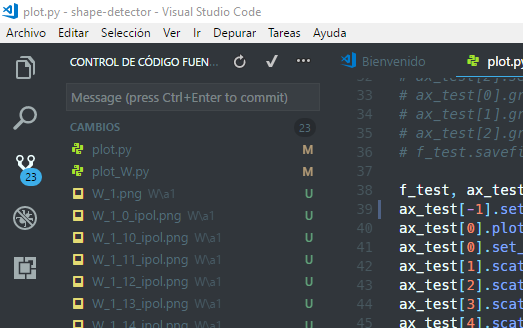
\includegraphics[width=0.9\textwidth]{fig/vscode_git.png}
		\end{column}
		\begin{column}[t]{0.5\textwidth}
			\textbf{Atom (Github)}
			\begin{itemize}
			\item Editor de código abierto
			\item Excelente integración con Github
			\end{itemize}

			\textbf{TortoiseGit} (para Windows)
			
			\textbf{ungit} (multiplataforma)
			
			\textbf{Github Desktop} (Win, Mac)
			
			\textbf{GitKraken} (multiplataforma)
			
			\hspace{1cm}$\vdots$
			
			\
			
			\url{https://git-scm.com/downloads/guis}
		\end{column}
	\end{columns}
\end{frame}

\begin{frame}[standout]\frametitle{TL;DR}
	\begin{itemize}
		\item Es libre
		\item Es cómodo
		\item Te da seguridad
		\item Es fácil de usar
		\item Es perfecto para nuestros trabajos
	\end{itemize}
\end{frame}

\end{document}
